% !TEX program = xelatex
\documentclass[tikz, crop, border = {2pt 2pt 2pt 2pt}]{standalone}

\usepackage{concmath-otf}
\usetikzlibrary{calc, angles, quotes, patterns}
\usetikzlibrary{decorations.pathreplacing, decorations.pathmorphing, calligraphy}

\begin{document}
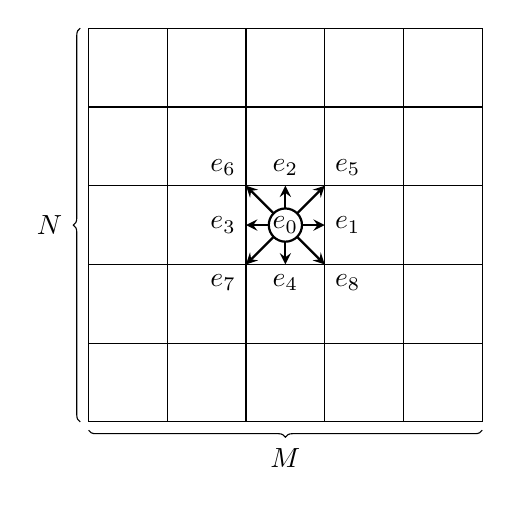
\begin{tikzpicture}
	\draw (0, 0) grid (5, 5);
	\draw[decorate, decoration = {brace, mirror, raise = 3pt}] (0, 0) -- node[below = 6pt]{$M$} (5, 0);
	\draw[decorate, decoration = {brace, raise = 3pt}] (0, 0) -- node[left = 6pt]{$N$} (0, 5);

	\def\cx{0, 1, 0, -1, 0, 1, -1, -1, 1}
	\def\cy{0, 0, 1, 0, -1, 1, 1, -1, -1}
	\def\coordlist{(0, 0), (1, 0), (0, 1), (-1, 0), (0, -1), (1, 1), (-1, 1), (-1, -1), (1, -1)}
	\def\coordlistnorm{(1/2, 0), (0, 1/2), (-1/2, 0), (0, -1/2), (1/2, 1/2), (-1/2, 1/2), (-1/2, -1/2), (1/2, -1/2)}

	\newcommand{\e}{\pmb{\symrm{e}}};
	% Drawing the vector part
	\coordinate (A) at (2.5, 2.5);
	\draw[-stealth, thick] (A) -- ++ (1/2, 0)    node[at end, right]{$\e_1$};
	\draw[-stealth, thick] (A) -- ++ (0, 1/2)    node[at end, above]{$\e_2$};
	\draw[-stealth, thick] (A) -- ++ (-1/2, 0)   node[at end, left]{$\e_3$};
	\draw[-stealth, thick] (A) -- ++ (0, -1/2)   node[at end, below]{$\e_4$};
	\draw[-stealth, thick] (A) -- ++ (1/2, 1/2)  node[at end, above right]{$\e_5$};
	\draw[-stealth, thick] (A) -- ++ (-1/2, 1/2) node[at end, above left]{$\e_6$};
	\draw[-stealth, thick] (A) -- ++ (-1/2, -1/2)node[at end, below left]{$\e_7$};
	\draw[-stealth, thick] (A) -- ++ (1/2, -1/2) node[at end, below right]{$\e_8$};

	\filldraw[fill = white, draw = black, thick] (A) circle (6pt) node{$\e_0$};
\end{tikzpicture}
\end{document}
